%%%%% COS 511 PROJECT REPORT

\documentclass[12pt]{article}

\usepackage{amsmath, amsfonts, amsthm, fullpage, amssymb, algpseudocode, algorithm, graphicx, multirow}

\setlength{\topmargin}{0pt}
\setlength{\textheight}{9in}
\setlength{\headheight}{0pt}
\setlength{\headsep}{0pt}
\setlength{\oddsidemargin}{0.25in}
\setlength{\textwidth}{6in}

\newcommand{\comment}[1]{}

\newtheorem{theorem}{Theorem}
\newtheorem{lemma}[theorem]{Lemma}
\newtheorem{invariant}[theorem]{Invariant}
\newtheorem{corollary}[theorem]{Corollary}
\newtheorem{definition}[theorem]{Definition}
\newtheorem{property}[theorem]{Property}
\newtheorem{remark}[theorem]{Remark}

\pagestyle{plain}

\begin{document}

\thispagestyle{empty}

%\begin{center}
%\bf\large COS 511: Theoretical Machine Learning
%\end{center}

\noindent
Lecturer: Rob Schapire   %%% FILL IN LECTURER (if not RS)
\hfill
Project Report              %%% FILL IN LECTURE NUMBER HERE
\\
Authors: Christian Eubank, Sachin Ravi                %%% FILL IN YOUR NAME HERE
\hfill
May 14, 2013           %%% FILL IN LECTURE DATE HERE

\noindent
\rule{\textwidth}{1pt}

\begin{center}
\bf\large Building a More Robust Poker Algorithm for the Multi-Armed Bandit Problem
\end{center}

\medskip

\section{Introduction}

We study the stochastic multi-armed bandit problem and present robust modifications to existing algorithms. In the bandit problem, a player is  
faced with a row of slot machines (``arms'') and during each round of the game pulls a single arm.  When chosen by the player, an arm provides a random reward according to its machine-specific distribution. The player's goal is to maximize the sum of rewards received through a
sequence of selections.  

An agent playing the bandit game is faced with the classic exploration-exploitation tradeoff.  On the one hand, the agent will want to 
exploit the best arm he has found so far by repeatedly pulling it. On the other hand, he could explore other arms,
which may or may not offer a higher reward.

Although the original motivation for the problem, which continues to be relevant (e.g. \cite{Cassell}), was scheduling clinical trials, many 
new applications have arisen.  One application is in ad placement, in which pulling an arm represents displaying an ad which, in turn,
provides some financial reward.  In \cite{Chakrabarti}, the authors formulate a modified version
of the problem where arms have a lifetime after which they expire. This expiration helps to model ads, which often 
have limited lifetimes due to their content and campaign budgets.  Another application is in Web document ranking 
in which, given a user's query, a site seeks to optimally rank and display relevant documents.
In \cite{Radlinski}, the authors propose an online learning method using multi-armed bandit algorithms that produces rankings from usage data.   

\section{Background}
Formally, the multi-armed bandit problem consists of a set of $K$ probability distributions
$(D_1, \ldots, D_k)$ with associated expected values $(\mu_1, \ldots, \mu_k)$.
Initially, the distributions $D_i$ are unknown to the player.  At each round $t = 1,2,\ldots,T$, the player selects an arm with index $j(t)$
and receives a reward $r(t) \sim D_{j(t)}$. The player's goal is to maximize his received reward summed over all rounds.  A bandit algorithm
specifies a strategy by which the player should choose an arm $j(t)$ in each round.

According to \cite{Kuleshov}, the most popular performance measure for bandit algorithms is \emph{total expected regret}.  Assuming the 
total number of rounds is $T$, \emph{total expected regret} is defined as
$$
R_T = T\mu^{*} - \sum_{i=1}^{T} \mu_{j(t)},
$$
where $\mu^{*} = \max(\mu_1, \ldots, \mu_k)$ is the expected reward from the best arm. 

As background for our approach to the problem, we present three pre-existing bandit algorithms: $\epsilon$-greedy, Boltzmann exploration and Poker.
For the next two subsections, let $p_i(t)$ be the probability of picking arm $i$ at time $t$.

\subsection{$\epsilon$-greedy}

The $\epsilon$-greedy algorithm is an extremely simple heuristic. \cite{Auer} refer to prior results guaranteeing that bandit algorithms will provide at least a logarithmic level of regret and note that a greedy approach with a dynamic value of $\epsilon$ can provide a polylogarithmic guarantee.

At each round $t = 1, \ldots, T$, the algorithm selects the arm with the highest observed empirical mean with probability $1 - \epsilon$ and
selects a random arm with probability $\epsilon$.  More specifically, given empirical means $\hat{\mu}_1, \ldots, \hat{\mu}_k$,
\begin{align*}
p_i(t+1) = 
\begin{cases}
1 - \epsilon + \frac{\epsilon}{k}, & \textrm{if } i = \arg \max_{j = 1, \ldots, k} \hat{\mu}_j(t) \\
\frac{\epsilon}{k}, & \textrm{otherwise}
\end{cases}
\end{align*}

Smaller values of the parameter $\epsilon$ will cause less exploration and more exploitation whereas larger values lead to comparatively more exploration. 

\subsection{Boltzmann Exploration}
While the $\epsilon$-greedy method explores by uniformly picking an arm at random, one instead might want the probability of an arm being chosen to be proportional to its observed reward. Intuitively, such an approach leverages a greater amount of information during the exploration phase.
The Boltzmann Exploration algorithm randomly picks an arm according to a probability proportional to its average observed reward according to the Boltzmann distribution.  Specifically, given empirical means $\hat{\mu}_1, \ldots, \hat{\mu}_k$,
\begin{align*}
p_i(t+1) = \frac{e^{\hat{\mu}_i(t)/\tau}}{\sum_{j=1}^{k} e^{\hat{\mu}_j(t)/\tau}} \, \, \textrm{for } i = 1, \ldots, k
\end{align*}

The value of $\tau$ (often called the ``temperature'' parameter) controls the randomness of the choices.  When $\tau \to 0$, the algorithm always greedily chooses the arm with the highest observed empirical average while when $\tau \to \infty$, the algorithm picks
arms uniformly at random. \cite{Kuleshov} notes that while a dynamic $\tau$ provides a polylogarthmic regret bound, running the algorithm with a static $\tau$ typically performs just as well.

\subsection{Poker}
The ``Price of Knowledge and Estimated Reward'' (Poker) strategy is a newer algorithm introduced in \cite{Mohri}.  Unlike the previous strategies,
Poker is a pricing strategy that assigns prices to each arm and at each round picks the arm that has the highest price.  The price for each arm 
takes into account the sample mean and variance data as well as the time horizon of the algorithm

Let $\mu^{*} = \max(\mu_1, \ldots, \mu_k)$ be the the highest mean.  Supposing $j_{0}$ is the index of the arm with the highest observed empirical mean, 
let $\hat{\mu}^{*} = \mu_{j_{0}}$ be the actual reward mean of this arm.
We know $\mu^{*} \ge \hat{\mu}^{*}$ and so $\mu^{*} - \hat{\mu}^{*}$ is a non-negative quantity.  We then denote 
$\delta_{\mu} = \mathbb{E}[\mu^{*} - \hat{\mu}^{*}]$ to be the expected reward improvement.

At each round, the expected gain when pulling an arm $i$ is given by the expected reward improvement $\delta_{\mu}$ multiplied by the probability of an
improvement $\Pr[\mu_i - \hat{\mu}^{*} \ge \delta_{\mu}]$, where $\mu_i$ is the reward actual mean of the arm $i$.  If we let $H$ be the number of remaining rounds, 
we can exploit this knowledge gain $H$ times and price arm $i$ at
$$
p_i = \hat{\mu}_i + \Pr[\mu_i - \hat{\mu}^{*} \ge \delta_{\mu}] \delta_{\mu} H,
$$
where $\hat{\mu}_i$ (the empirical average) represents the exploitation price and the second term represents the exploration price of arm $i$. 

Let us now discuss the calculation of the second term.  Suppose $\hat{\mu}_{i_1} > \ldots > \hat{\mu}_{i_q}$ be the ordered observed means of arms.  
We let $\delta_u = \left(\hat{\mu}_{i_1} - \hat{\mu}_{i_{\sqrt{q}}} \right)/\sqrt{q}$.  The authors chose $\sqrt{q}$ here because they observe that it works well
in practice and minimizes variance and bias.

Let $\mathcal{N}(x, \mu, \sigma) = \frac{1}{\sqrt{2 \pi \sigma}} \exp \left(\frac{(x - \mu)^2}{2 \sigma^2} \right)$ be the normal distribution.  
Let $\hat{\mu}_i$ be the observed mean estimate, $\hat{\sigma}_i$ be the standard deviation estimate, and $n_i$ be the number of times the arm has been chosen, then
we say (noting that the equality is exact if $\hat{\mu}_{i}$ is normally distributed)
$$
\Pr[\mu_i \ge \hat{\mu}^{*} + \delta_u] \approx \int_{\hat{\mu}^{*} + \delta_{\mu}}^{\infty} \mathcal{N}\left(x, \hat{\mu}_{i}, \frac{\hat{\sigma}_i}{\sqrt{n_i}} \right) dx.
$$

\begin{algorithm}
\scriptsize
  \caption{Pseudocode for Poker Algorithm}
  \begin{algorithmic}
  \State $\forall i, \, \, N[i] \gets 0$ \Comment{Stores the number of times an arm has been pulled}
  \State $\forall i, \, \, \mu[i] \gets 0$ \Comment{Stores the empirical mean for each arm}
  \State $\forall i, \, \, \sigma[i] \gets 0$ \Comment{Stores the empirical standard deviation for each arm}
  \State
  \State Pick two different random arms twice each; update $\mu$, $\sigma$, and $N$
    \For{$t = 5$ to $T$}
    	\State $p_{max} \gets -\infty$
        \State $q \gets |\{i \, : \, N[i] > 0\}|$
        \State $i_{*} \gets \arg \max_{i} \{\mu[i]\}$
        \State $i_{\sqrt{q}} \gets j$ s.t. $|\{i : u[i] > u[j]\}| = \sqrt{q}$
        \State $\delta_{\mu} \gets \frac{\mu[i_{*}] - \mu[i_{\sqrt{q}}]}{\sqrt{q}}$ 
        \For{$i = 1$ to $K$}
            \If{$N[i] > 0$}
               \State $\bar{\mu} \gets \mu[i]$ 
            \Else 
                \State $\bar{\mu} \gets \texttt{AVG}(\mu)$ 
            \EndIf
            \If{$N[i] > 1$}
                    \State $\bar{\sigma} \gets {\sigma[i] \over{\sqrt{N[i]}}}$
            \Else
               \State $\bar{\sigma} \gets \texttt{AVG}(\sigma)$ 
            \EndIf
        \State $p \gets \bar{\mu} + \delta_{\mu}(T - t) + \int_{\mu[i_*] + \delta_{\mu}}^{\infty} \mathcal{N}\left(x, \bar{\mu}, \bar{\sigma} \right) dx$
        \If{$p > p_{max}$} 
            \State$p_{max} \gets p$
            \State $i_{max} \gets i$ 
        \EndIf
        \EndFor
        \State Pick arm $i_{max}$, receive reward $r$ and update $\mu$, $\sigma$, and $N$ accordingly
    \EndFor
  \end{algorithmic}
\end{algorithm}


\section{New Algorithms}

\subsection{Motivation}

The authors' proof that Poker is a zero regret strategy hinges upon considering infinite horizons and considering the behavior of the price functions as $H$ approaches infinity.\footnote{The authors specifically seek to prove that there does not exist a lever that provides high regret that is pulled many times by the algorithm with a non-trivial probability.} However, in practice the value of $H$ will be finite either due to the fact that the number of rounds is known in advance or, as the authors suggest in the case in which the number of rounds is unknown, the algorithm treats $H$ as a fixed parameter.

Recall Poker initializes itself by pulling two random arms twice. We present a simple bandit instance that will cause Poker to perform extremely poorly with a nontrivial probability.

We define the bandit instance $\texttt{PATHOLOGICAL}(p)$ for $p \in [0,1]$ as a set of $K$ levers with mean rewards in $[0,1]$. We consider $(1-p)$ levers to be good (i.e. they all have mean rewards of 1) and the other $p$ levers to be bad. We consider the bad levers to have equally spaced rewards in the range $[0,\gamma]$ for some constant $\gamma$. Finally, we assume all levers provide normally-distributed payoffs with the same standard deviation $\sigma$. \\

\noindent
\textbf{Claim} For a finite $H$, as $\sigma \rightarrow 0$, the probability that Poker running on $\texttt{PATHOLOGICAL}(p)$ will lead to a choice of arms with nearly the maximum possible regret (i.e. at least $(1-\gamma)$) each round is $O(p^{2})$. \\ 

Suppose that Poker initially chooses to pull two distinct bad arms. We require the two bad arms to be distinct. If the two arms were the same, all $\hat{\mu}_{i}$ and $\hat{\sigma}_{i}$ would be equal and the following argument would fail. Without loss of generality, let the indices of these arms be 1 and 2. By this point, the algorithm will have calculated $\hat{\mu}_{1}, \hat{\mu}_{2}, \hat{\sigma}_{1},\hat{\sigma}_{2}$ and, for all $i > 2$, will have set $\hat{\mu}_{i}= {\hat{\mu}_{1}+\hat{\mu}_{2}\over 2}$ and $\hat{\sigma}_{i} = {\hat{\sigma}_{1}+\hat{\sigma}_{2}\over 2}$

In each turn, the algorithm sets $p_{i} = \hat{\mu}_{i} + \delta_{\mu}(T-t)\int_{\mu^{*}+\delta_{\mu}}^{\infty}\mathcal{N}(x,\hat{\mu}_{i}, \hat{\sigma}_{i})dx$

We have assumed that $H$ is finite and, by definition $\delta_{m}$ will be finite. With respect $\int_{\mu^{*}+\delta_{\mu}}^{\infty}\mathcal{N}(x,\hat{\mu}_{i}, \hat{\sigma}_{i})dx$, for all $i$, $\mu^{*}+\delta_{\mu}$ will be greater than $\mu_{i}$. As a result, as $\sigma \to 0$, $\hat{\sigma}_{i} \to 0$ and the value of the integral also converges to 0.

Thus, if $\sigma$ is arbitrarily close to $0$, $p_{i} \rightarrow \hat{\mu}_{i}$ and Poker will continue to greedily pick the lever with the highest empirical mean. Given that the unobserved levers have empirical means set equal to the average of the empirical means of levers 1 and 2, one of the levers pulled during initialization will have a strictly greater empirical mean.\footnote{We are ignoring the case that $\hat{\mu}_{1} = \hat{\mu}_{2}$ exactly because since the rewards are real numbers and their true means are different, the probability of this strict equality holding is 0}

As a result, the algorithm initialized with two bad arms will greedily keep playing one of these two bad arms for the entire time frame. Give that the maximum payout is 1 and the best payout of any bad arm is $\gamma$, the expected regret per round will be at least $1-\gamma$. 

Finally, the probability that Poker initializes by choosing two distinct bad arms is simply $({pK\over{K}})({p(K-1)\over{K}}) = ({K-1\over K})p^{2}$ desired.

\subsection{Our approach}

While the pathological distribution used in our worst-case analysis of Poker may be a somewhat artificial example, it demonstrates that in cases in which the arms' reward variances are small, the algorithm's final choices of arms could be highly dependent  on the initial choice of arms. An obvious solution to this problem is to simply initialize the algorithm with a greater number of random arms. However, we instead opted to merge the Poker algorithm with algorithms that incorporate a greater degree of randomness.

A logical extension to the Poker algorithm is \texttt{greedyPoker} in which, at each round (other than the initialization rounds), we pull a random lever with probability $\epsilon$. Otherwise, we pick the arm with the highest value of $p_{i}$. As $\epsilon \to 0$, \texttt{greedyPoker} converges to standard Poker and as $\epsilon \to 1$, the algorithm converges to guessing.

Likewise, we consider merging Poker with the Boltzmann algorithm. During each round $\texttt{boltzPoker}$, the algorithm calculates the vector of $p_{i}$ values. Next, the algorithm maps this vector of values into probabilities in accordance to the Boltzmann distribution and a temperature parameter. The algorithm then chooses the arm to pull based on this distribution.\footnote{In terms of implementation, we first normalize the vector of $p_{i}$ such that all the entries lie in $[0,1]$ so as to avoid numerical overflow during the calculations.} As the temperature parameter $\tau \to 0$, \texttt{boltzPoker} acts like the standard Poker algorithm while as $\tau \to \infty$, the algorithm converges to random guessing.

In terms of design, we anticipated that the modified algorithms would be more robust in dealing with the initial conditions when compared to Poker due to the incorporation of additional randomness. Likewise,  we also believed that $p_{i}$ values, which incorporate information regarding the standard deviations and time horizon, should be a superior proxy for the ``goodness" of arms as compared to the sample means used in the basic Boltzmann and $\epsilon$-greedy algorithms.

In terms of theoretical performance, we can set the algorithms' parameters to be such that they will act as if they were simply the standard Poker algorithm. By manipulating the parameters, we can guarantee that the algorithms will perform at least as well as the standard Poker algorithm. However, finding these ideal parameters for every distribution (assuming they exist) is not necessarily a trivial task and requires extensive experimentation.

\section{Experiments}

We evaluate the strategies using four datasets: three generated artificially using the Normal, Inverse-Gaussian and Gumbel distributions, respectively,
and one that is a real networking dataset that was also used for evaluation in \cite{Mohri}.  The networking dataset details the retrieval latency of more than $700$
universities as sources for every $10$ min for about $10$ days ($\sim 1300$ rounds).  Each page is thus associated with an arm and each latency is associated to a negative reward.
We implemented each of the algorithms mentioned above in Python.\footnote{We have made all our code available at \texttt{https://github.com/cgeubank/COS511-BanditProject}}

For the algorithms that need parameters as inputs, we determined the value of these parameters by tuning them on a dataset generated by the Normal distribution, with $100$ arms,
with $1000$ rounds, and averaged over 25 trials/ distribution instances.  Please refer to Figure~\ref{fig:tuning} for more information about the specific parameters used.  We found that the choice of parameters
were roughly equal when tuning them on the other artificial distributions.

\begin{figure}
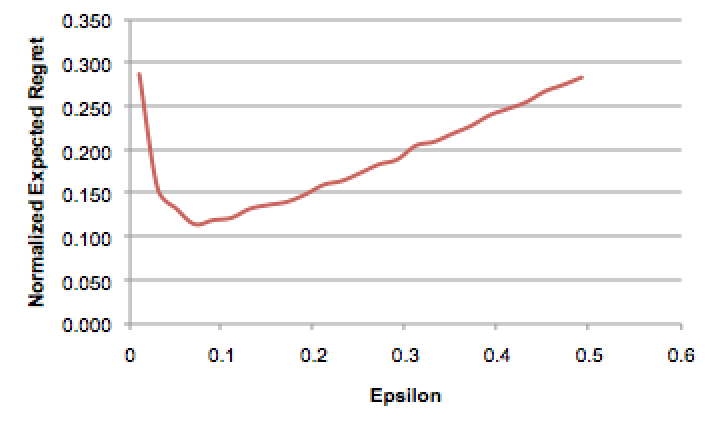
\includegraphics[width=0.5\textwidth]{EpsilonTuning}
\hfill
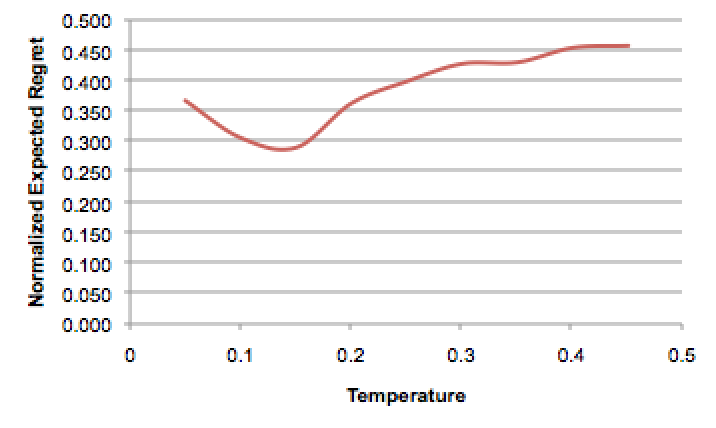
\includegraphics[width=0.5\textwidth]{TempTuning}
\caption{Tuning data used to find $\epsilon$ and $\tau$ values for $\epsilon$-Greedy and Boltzmann algorithms, respectively.  The data for \texttt{greedyPoker} and \texttt{boltzPoker} followed the same trend and have thus been omitted for readability.}
\label{fig:tuning}
\end{figure}

In the experiments, the \texttt{Random} strategy involves picking an arm uniformly at random in each round and is used to provide a baseline for the results.  Additionally,
rather than measure the performance in terms of each strategy's expected regret, we normalize the expected regret as a percent of the maximum possible expected regret so as to get a value in $[0,1]$. 

\subsection{Performance on Datasets}
For each specific distribution, the data was generated by picking the mean and standard deviation (or in the case of Gumbel, $\beta$ value) uniformly at random from $[0,1]$.  The choice of what
distributions to use was based on the fact that these distributions were also tested in \cite{Kuleshov}. 

For the three randomized distributions, $\epsilon$-greedy performs surprising well, when compared to the Boltzmann and \texttt{boltzPoker} algorithms.  Especially after tuning, 
\texttt{greedyPoker} performed the best on the three datasets, achieving nearly a third of the expected regret as Poker on Gumbel.  On the other hand, Poker performed second-best
on the Normal and Inverse-Gaussian distributions despite having no parameters to tune.

Having tuned the algorithms, we expected that these optimal parameters would allow them to also perform favorably on the real-world network dataset. However, we found that
the Poker algorithm significantly outperformed the other algorithms, including \texttt{boltzPoker} by greater than a factor of 5. Later, we were able to tune the parameters
to get \texttt{greedyPoker} to perform marginally better than Poker on the dataset. However, this tuning required hundreds of trial runs while Poker achieved its performance
without any kind of tuning.\footnote{More pessimistically, while we could lower $\epsilon$ to an arbitrarily small level, reducing $\tau$ to below 0.005 in \texttt{boltzPoker} led to the risk of numerical overflow in the $e^{\mu / \tau}$ terms.} In real world situations, a user may not have access to the data sets or time to tune parameters before facing a bandit instance.

\begin{table}[htbp]
  \centering
  \caption{Normalized Expected Regret on Datasets with Optimally-Tuned Parameters}
    \begin{tabular}{|c|c|c|c|c|}
    \hline
    \multicolumn{1}{|c|}{\multirow{2}[5]{*}{\textbf{Algorithm}}} & \multicolumn{4}{|c|}{\textbf{Distribution}} \\ \cline{2-5}
    \multicolumn{1}{|c|}{} & \multicolumn{1}{|c|}{\textbf{Normal}} & \multicolumn{1}{|c|}{\textbf{Inverse Gaussian}} & \multicolumn{1}{|c|}{\textbf{Gumbel}} & \multicolumn{1}{|c|}{\textbf{Networking}} \\ \hline
    \multicolumn{1}{|l|}{\textbf{$\epsilon$-greedy}} & 0.129 & 0.152 & 0.092 & 0.034 \\  \hline
    \multicolumn{1}{|l|}{\texttt{greedyPoker}} & 0.077 & 0.081 & 0.052 & 0.012   \\ \hline
    \multicolumn{1}{|l|}{\textbf{Poker}} & 0.101 & 0.108 & 0.139  & 0.007\\ \hline
    \multicolumn{1}{|l|}{\textbf{Boltzmann}} & 0.151 & 0.109 & 0.134 & 0.029  \\ \hline
    \multicolumn{1}{|l|}{\texttt{boltzPoker}} & 0.177 & 0.116 & 0.133  & 0.038 \\ \hline
    \multicolumn{1}{|l|}{\texttt{Random}} & 0.278 & 0.292 & 0.316 & 0.041  \\ \hline
    \end{tabular}%
  \label{tab:tuned_results}%
\end{table}%


\section{Conclusion}

We present two canonical algorithms for the multi-armed bandit problem as well as Poker, a newer algorithm that incorporates the time horizons of particular bandit instances as well as the sample standard deviations into its analysis. We identify a theoretical weakness in the initialization process of the Poker algorithm and merge Poker with the other two algorithms to create more robust versions of the algorithm.

After tuning the parameters for these algorithms, we find that \texttt{greedyPoker} in particular has a stronger performance than the Poker algorithm on random instances based on the Normal, Inverse Gaussian and Gumbel distribution. However, when using these algorithms on real data with the same tuned parameters, the standard Poker algorithm had a much better performance.

Overall, while the modified algorithms we created have at least as good performance when compared to the standard Poker algorithm given the correct tuning parameters. Hence, against certain instances in which these tuning parameters are already known, these algorithms may present a superior level of expected regret. However, on real distributions whose properties are not known, the standard Poker algorithm may be theoretically more vulnerable with respect to its initial conditions but appears to have a consistently strong performance in practice.

\bibliographystyle{plain}
\bibliography{references}

\end{document}
